\chapter{Adaptive Large Neighbourhood Search}

The Adaptive Large Neighbourhood Search (ALNS) is an alternative method that can be used to solve the bunker supply problem. The outline for ALNS is defined in Algorithm \ref{Algo_1}.

In line \ref{Al1:L1}, an initial solution is first constructed before the main ALNS algorithm is applied to find a good solution. The Nearest Neighbour heuristic used to create an initial route $s_{initial}$. This would be set as the candidate route $s$.

Subsequently, the candidate route $s$ would undergo destroy and repair operations to create a new route $s'$. A destroy operator $d$ is chosen from a set of destroy operators $d()$. An operator is chosen probabilistically from its weights $w_{d}$, with higher weighted operators having a higher likelihood of being chosen. At the start, weights of all operators would be equal. The same procedure is done to chose repair operator $r$ from the set of repair operators $r()$ using weights $w_{r}$. The new route $s'$ is then evaluated against $s$ and accepted to be the next candidate route according to the acceptance criteria. Otherwise the new route $s'$ is discarded. This cycle repeats until the stopping criteria is reached. During this process, the best found route so far is recorded as $s_{max}$. The creation of an initial route and 2 iterations of the repair and destroy process is illustrated in Figure \ref{Fig:Destroy_and_Repair}.

\begin{figure} 
\begin{subfigure}{\textwidth}
	\centering
	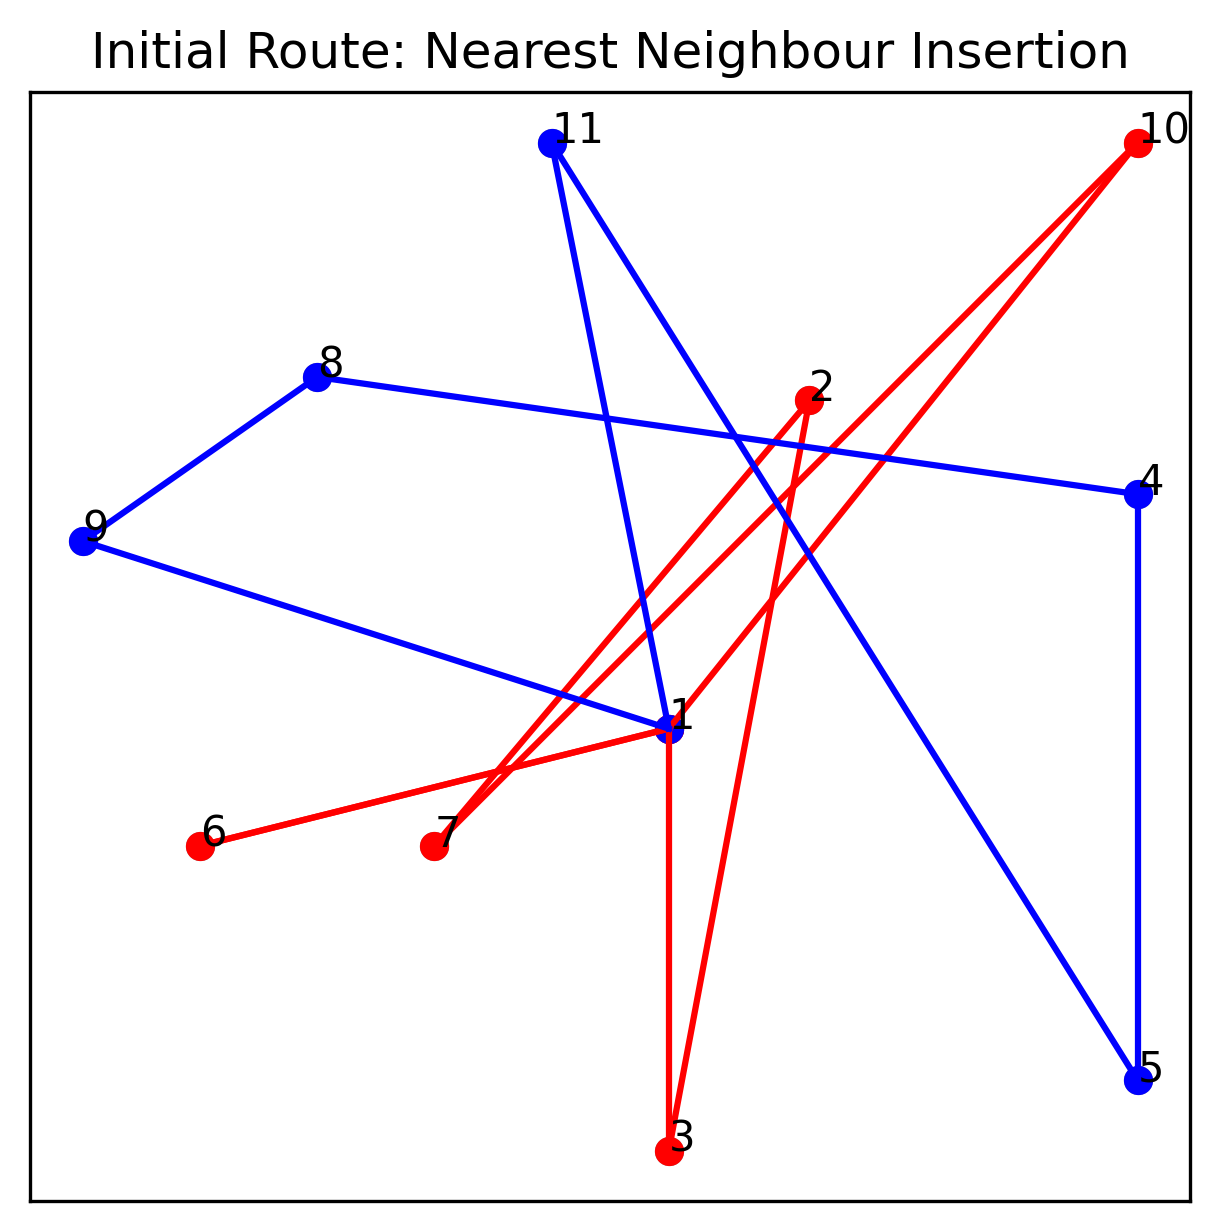
\includegraphics[scale=0.7]{R211_1.png}
\end{subfigure}

\begin{subfigure}{.5\textwidth}
	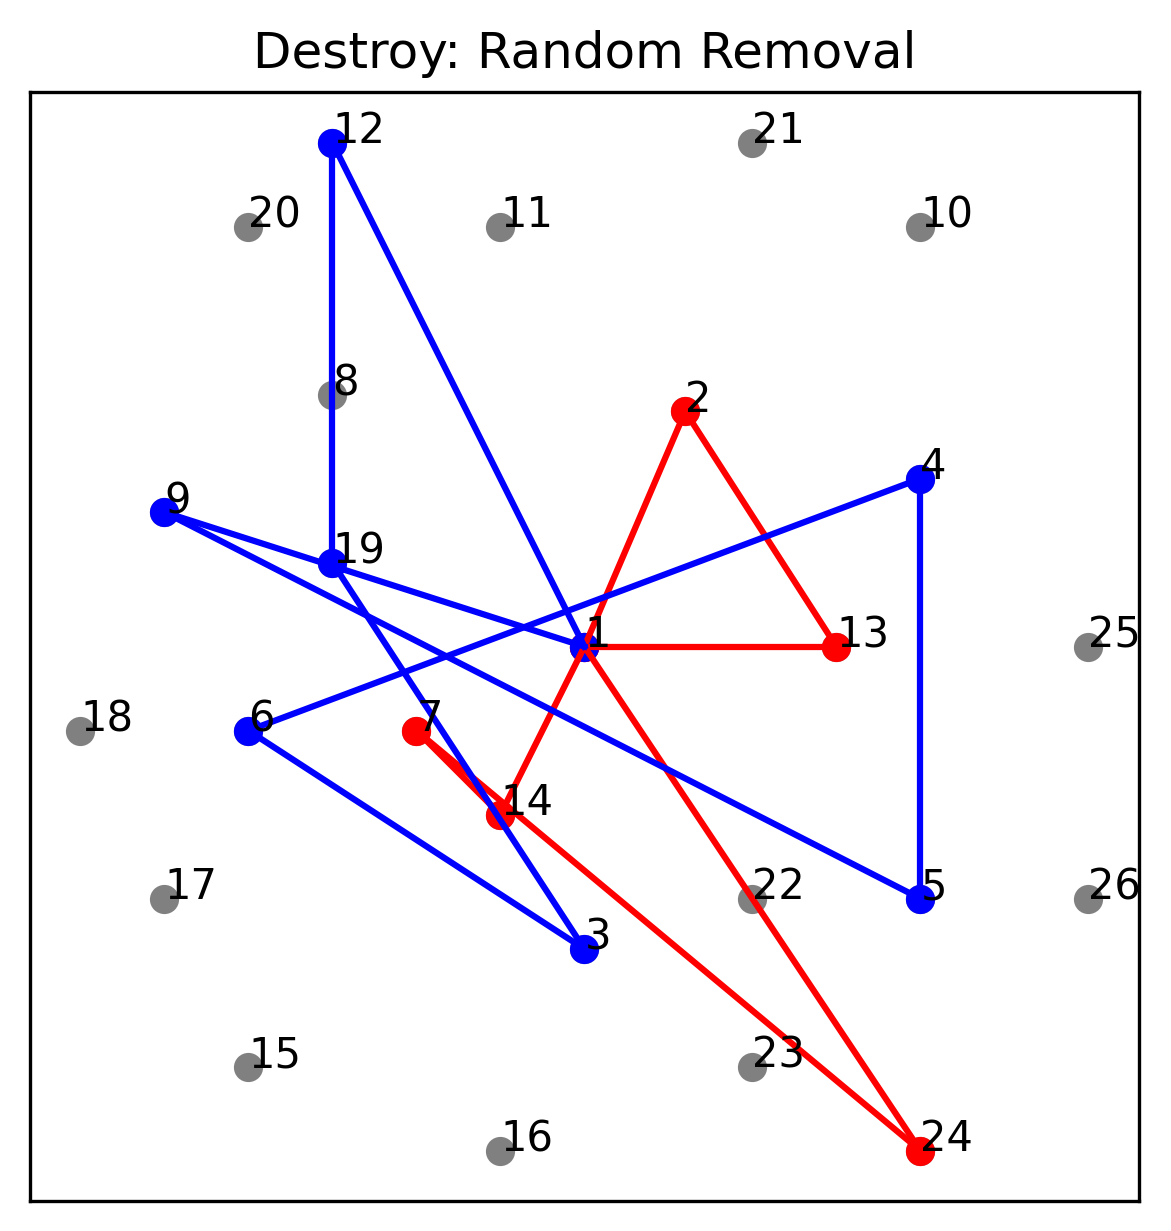
\includegraphics[scale=0.7]{R211_2.png}
\end{subfigure}
\begin{subfigure}{.5\textwidth}
	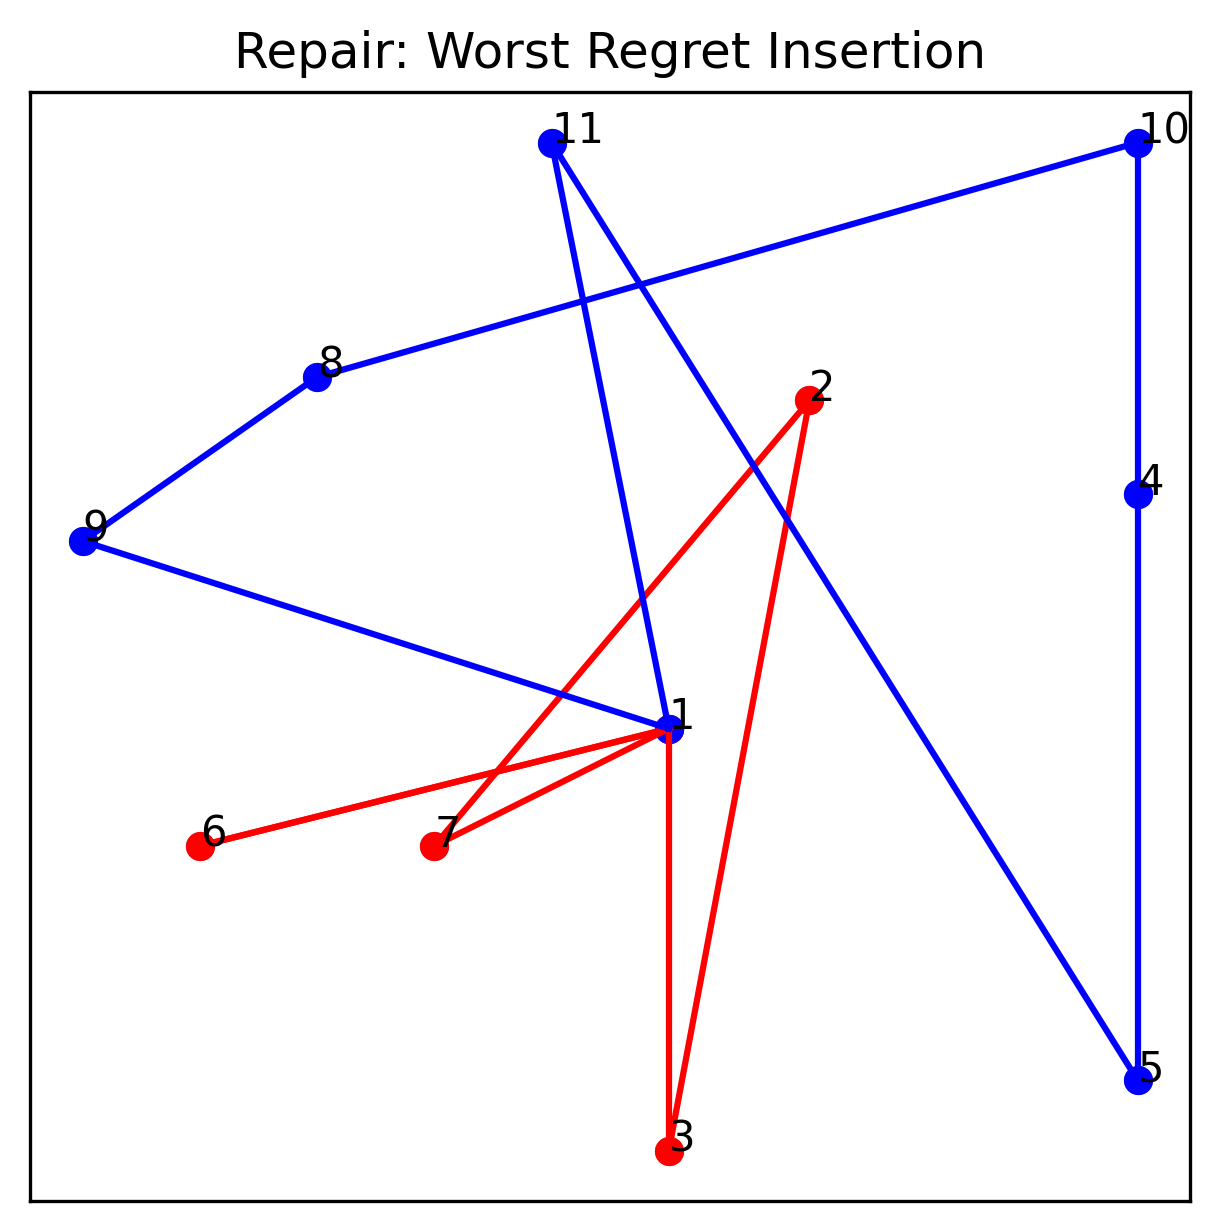
\includegraphics[scale=0.7]{R211_3.png}
\end{subfigure}

\begin{subfigure}{.5\textwidth}
	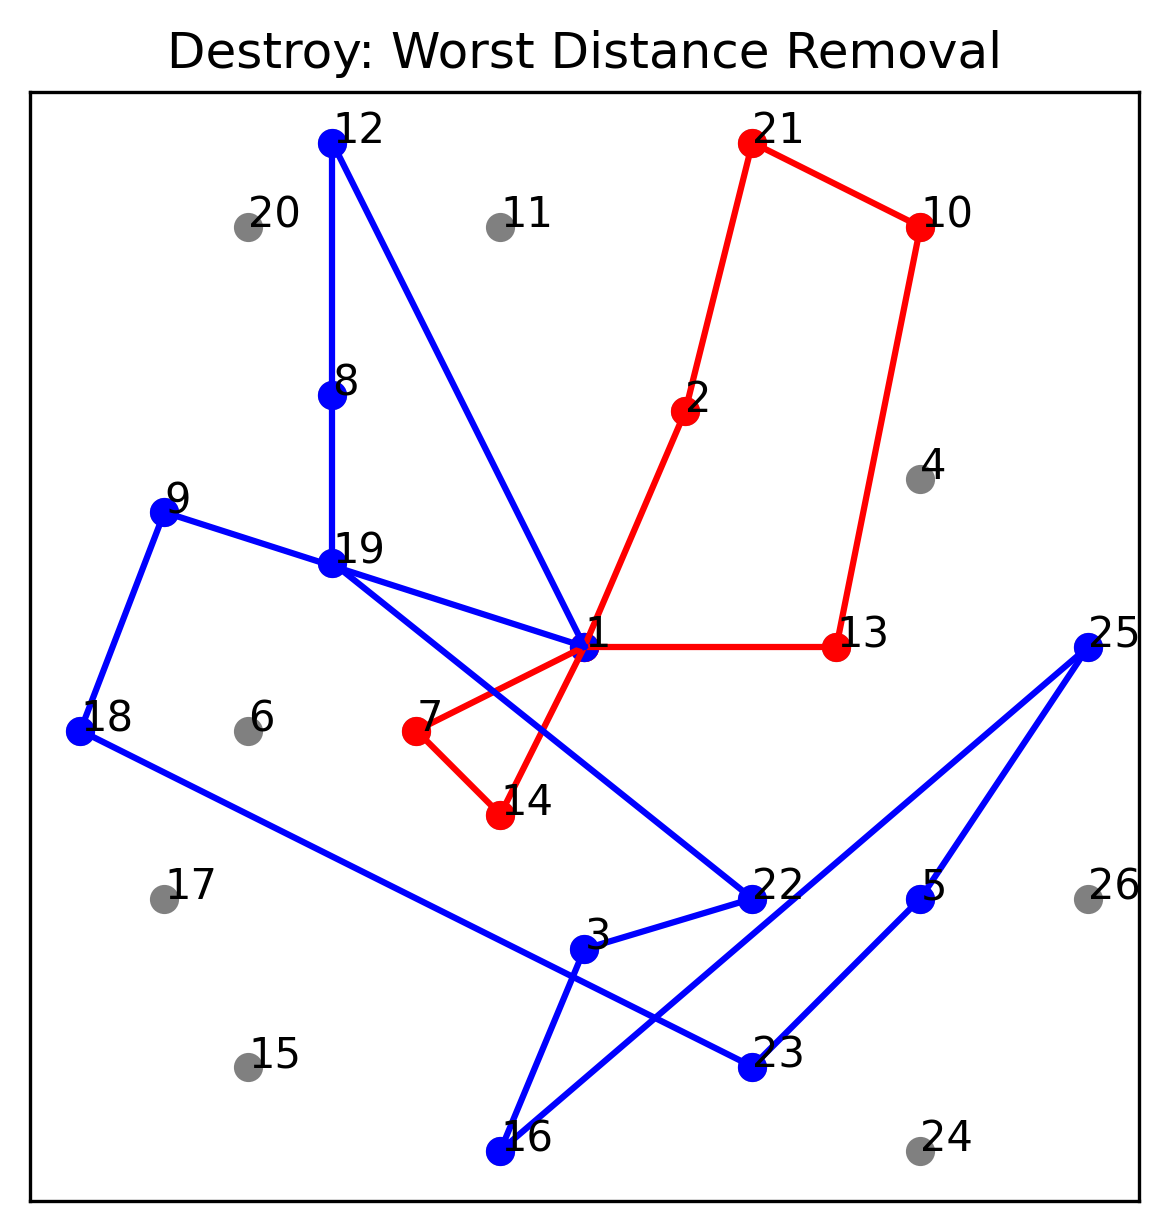
\includegraphics[scale=0.7]{R211_4.png}
\end{subfigure}
\begin{subfigure}{.5\textwidth}
	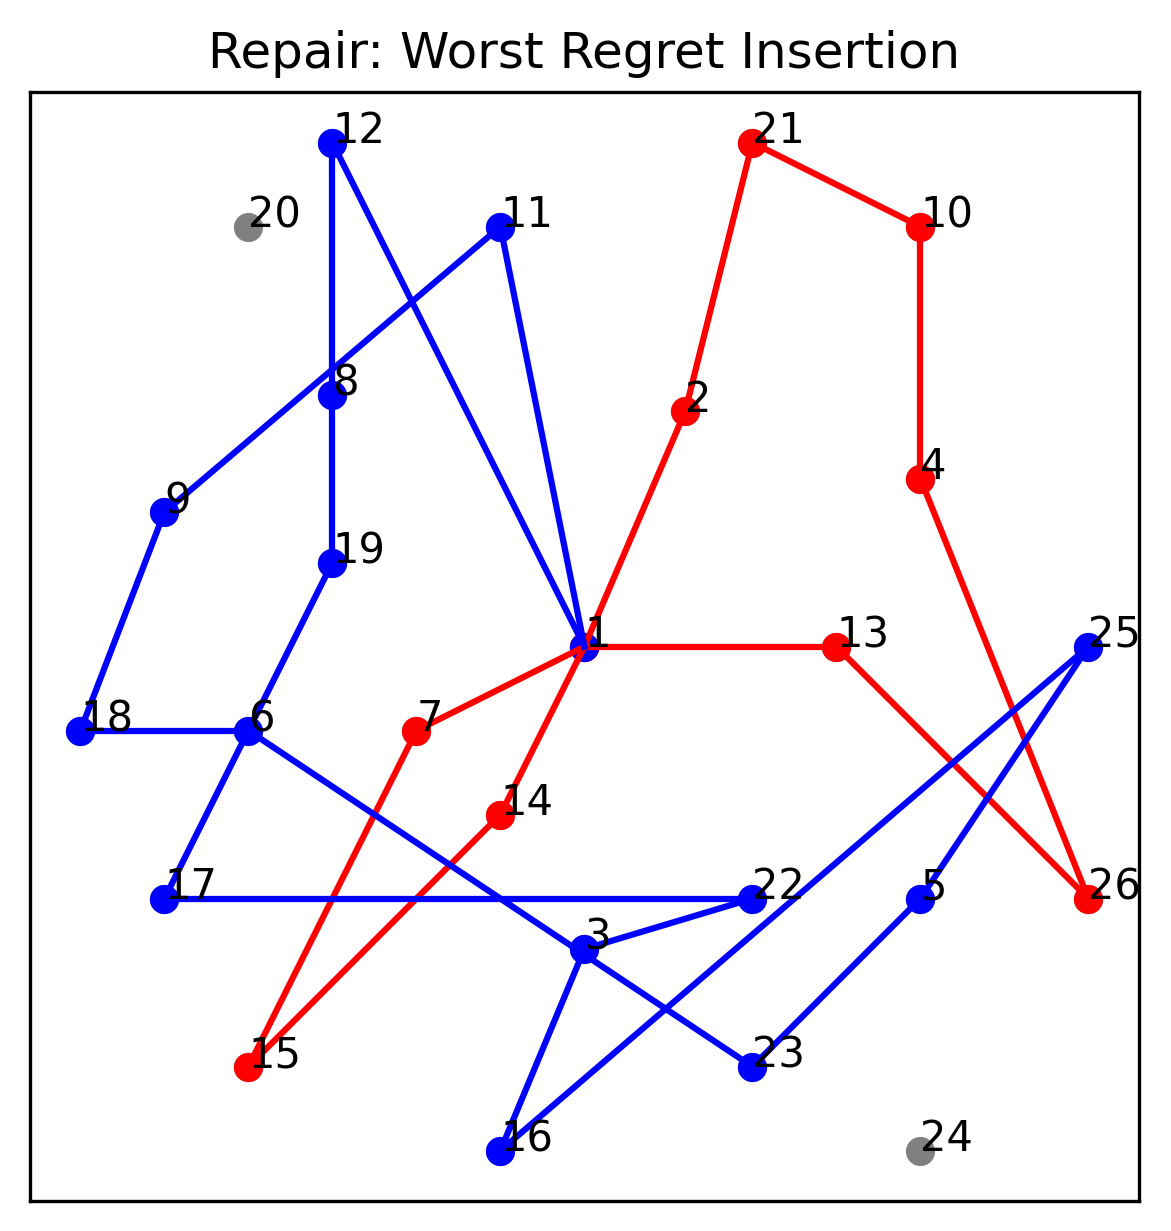
\includegraphics[scale=0.7]{R211_5.png}
\end{subfigure}
\caption{Creation of initial route and repair and destroy process} \label{Fig:Destroy_and_Repair}
\end{figure} 

The weights for the destroy and repair operators are updated according to their performance, controlled by the learning rate $l_{r}$ parameter. It is assumed that past performance is indicative of future performance. As such weights of well performing operators are increased to make it more likely for them to be chosen in subsequent iterations, improving the performance of the overall algorithm. Such a mechanism is in place as it is unknown which operator would work best for a given problem structure (tight time windows/ many unserved customers etc.). Thus, several operators are implemented and chosen from to allow the overall algorithm to have good performance across different problem structures. 

A range of destroy and repair operators are implemented such that there is a balance of diversifying and intensifying operators. Diversifying operators are those which allow the solution to explore new regions in the search space while intensifying operators focus on improving the solution in a local region.

This process continues until the stopping criteria is met. The stopping criteria is reached when the temperature $\mathcal{T}$ reaches 0 or a certain number of non-improving steps is reached.

\begin{algorithm} 
\SetKwFunction{InitialSolution}{InitialSolution}
\SetKwInOut{Input}{input}\SetKwInOut{Output}{output}
\Input{ProblemIinstance $i$}
\Output{Best Solution $s_{max}$}
\BlankLine
$s \leftarrow$ \InitialSolution{$i$}\; \label{Al1:L1}
$s_{max} \leftarrow s$\;
\While{stopping criteria not met}{

	%\For{$i\leftarrow 1$ \KwTo $p_{u}$}{
		select destroy method $d()$ and repair method $r()$ from $w_{d}, w_{r}$\;
		$s' \gets r(d(s))$\;
		 \If{accept($s, s'$)}{
            $s \gets s'$\;
            \If{$c(s) < c(s_{max})$}{
                $s_{max} \gets s$\;
            }
           }
        update $w_{d}, w_{r}$\;
	%}
}
\caption{Adaptive Large Neighbourhood Search} \label{Algo_1}
\end{algorithm} 

\section{Acceptance Criteria} \label{sec:SA}
The acceptance algorithm, Simulated Annealing (SA), is inspired from a physical process in metallurgy known as annealing. Temperature, $\mathcal{T}$, is used to control the randomness allowed during the search. At the start of the iteration, the process would start at a high temperature $\mathcal{T}$ value, which reduces according to the cooling schedule for each subsequent iteration. During each iteration, a new route $s'$ is created from the candidate route $s$. If  $s'$ is better than $s$, it is accepted as the new candidate route. However, if $s'$ is worse, it may be accepted as the new candidate route according to the Metropolis criteria as defined by equation \ref{eq:SA}.

\NewEnviron{HUGE}{% 
    \scalebox{1.3}{$\BODY$} 
} 
\begin{equation} \label{eq:SA} \HUGE
e^{\frac{f(s')-f(s)}{\mathcal{T}}}
\end{equation}

Using the current temperature and the difference of the objective function of the new and candidate route, a threshold can be generated using equation \ref{eq:SA}. A random number between 0 and 1 is generated and compared to the threshold. If the random number is lower than the threshold, the poorer new route is accepted. Otherwise it is discarded and there is no change to the candidate route. 

As the temperature decreases, the threshold value also decreases. This decreases the probability that a poorer route is accepted and the search would converge to the local best route.

Thus, in high temperature regimes, the acceptance criteria acts like a random walk, where almost all solutions are accepted. In a low temperature regime, the criteria acts like a hill climb, with only improving solutions accepted.

Other alternative criteria may be used such as a pure hill climbing criteria, which only accepts a solution if it is better than the candidate solution. However, SA is chosen as it allows the algorithm to explore poorer solutions early in the iteration, which may have the potential to create better solutions after refinement. This prevents the algorithm from being stuck in a local maxima.

\subsection{Cooling Schedule}
For each iteration, a temperature variable $\mathcal{T}$ is recorded and updated for use in the SA acceptance criteria. $\mathcal{T}$ is initialised at a starting maximum temperature $\mathcal{T}_{max}$ and the algorithm ends when it reduces to below $\mathcal{T}_{min}$. At each iteration of the algorithm, $\mathcal{T}$ is adjusted according to:
\begin{equation}
\mathcal{T}_{i+1} = \alpha \mathcal{T}_{i}
\end{equation}
where $i$ refers to the iteration number and $\alpha$ is the pre-set cooling rate.

As such, the number of iterations $MaxIter$ needed for the algorithm to terminate is as follows:

\begin{equation}
MaxIter = \log_\alpha \frac{\mathcal{T}_{min}}{\mathcal{T}_{max}}
\end{equation}

Other than the exponential cooling schedule proposed, alternative schedules can also be implemented, such as the linear or logarithmic schedule, which would result in lesser or more exploration at later stages of the algorithm respectively. The exponential schedule is chosen as it is the most popular and provides a good balance between early exploration of good regions at the start of the algorithm and later explorations of the local minima towards the end of the algorithm.
\section{Operator Selection}
The destroy $d()$ and repair operators $r()$ are chosen using weights $w_{d}, w_{r}$ respectively using the roulette wheel mechanism. The probability of an operator $i$ being chosen is given by
\begin{equation} \label{eq:RW}
P(i) = \frac{w(i)} {\sum_{j=1}^{k} w(ij)}
\end{equation}

At the start, weights of all operators are initialised to 1. After each iteration, the weights are awarded a score $\sigma$ according to the Table \ref{tab:score_adjustment}. To ensure the scores are sensible, $\sigma_1 > \sigma_2 > \sigma_3 > \sigma_4$.

\begin{table}[h]
    \centering
    %\renewcommand{\arraystretch}{1.3} % Adjust row spacing
    \begin{tabular}{ll} 
        \toprule
        \textbf{Score} & \textbf{Description} \\ 
        \midrule
        $\sigma_1$ & The last iteration resulted in a new global best solution.\\ 
        
        $\sigma_2$ & The last iteration resulted in a solution that has not been \\ 
                   & accepted before. The cost of the new solution is better than \\ 
                   & the cost of the current solution.\\ 
                   
        $\sigma_3$ & The last iteration resulted in a solution that has not been \\ 
                   & accepted before. The cost of the new solution is worse than \\ 
                   & the cost of the current solution, but the solution was accepted. \\ 
                   
       	$\sigma_4$ & The last iteration resulted in a solution has been rejected.\\ 
                   & The cost of the new solution is worse than the cost of the\\ 
                   & current solution. \\ 
        \bottomrule
    \end{tabular}
    \caption{Score Adjustment Parameters}
    \label{tab:score_adjustment}
\end{table}

Subsequently, the weights of the operators used are adjusted every $N_{update}$ iterations. $N_{update}$ is defined using a $\theta_{update}$ parameter which sets $N_{update}$ as a fraction of $MaxIter$.

\begin{equation}
N_{update} = \theta_{update} *MaxIter
\end{equation}

At every $N_{update}$ iterations, the weights are updated as follows.
\begin{equation} \label{eq:AA}
w (i) = w(i) (1-l_{r}) + l_{r} \frac{\pi_{i}}{\beta_{i}}
\end{equation}
$l_{r}$ is a pre-set learning rate factor $0<l_{r}<1$. A value of 0 results in no adjustments of weights according to performance while a value of 1 would mean only the performance of the previous iteration is considered. $\pi_{i}$ is the sum of all scores $\sigma$ accumulated by the operator and $\beta_{i}$ is the number of times the operator is used during $N_{update}$ iterations.

\section{Nearest Neighbour Search}
In the Nearest Neighbour Search (NNS) the initial route is created by are adding customers which are closest from the previous visit. If addition of a customer exceeds the capacity for the trip, the customer is added to the next trip instead. This process ends when no more customers can be added to the route without exceeding the time windows. This is done until all vehicles are assigned a route.

In this implementation, the NNS is modified with the seed customer chosen to be furthest from the terminal, instead of closest to the terminal. This is done so that the route created would be moving closer towards the terminal, allowing for quick top-up of fuel if the barge needs to return back to the terminal.

Apart from NNS, other heuristics may be used to create an initial route. However, it is noted that the algorithm to produce an initial route is not intended to create a particularly optimised route. Speed and simplicity are prioritised over being able to create a good route.

\begin{algorithm} \label{Algo 2}
\SetKwFunction{FeasibleCheck}{FeasibleCheck}
\SetKwInOut{Input}{input}\SetKwInOut{Output}{output}
\Input{Problem Instance $i$}
\Output{Initial Solution $s_{initial}$}
\BlankLine

\For{$k \leftarrow 0$ \KwTo $N_{barges}$}{
	$s_{initial} \leftarrow i$ select furthest customer $i$\;
	\Repeat {unfeasible}{
	$j \leftarrow$ closest customer from last customer $i$ in $s_{initial}$\;
	$s'\leftarrow s_{initial} + j$ \;
	\If {\FeasibleCheck{$s'$}}{
	$s_{initial} \leftarrow s'$ 
	}
	}
}

\caption{Nearest Neighbour Search}
\end{algorithm}


\section{Destroy Operators}
The destroy operators take in a route and destroys it by removing customers. The number of customers removed is a random value between 1 and a pre-set maximum degree of destruction $\mathcal{D}$. To allow the algorithm to search a large neighbourhood, the maximum degree of destruction is usually set to a relatively large number. By destroying the route, we allow the removed customers to be reinserted later during the repair phase in a more favourable position or to remove inefficient customers and allow other customers to be served instead. Random Removal, Worst Distance Removal and Shaw Removal are 3 destroy operators that can be chosen.

\subsection{Random Removal}
The Random Removal (RR) operator randomly removes customers from a random barge and trip from the route. This allows for some randomness in the heuristic, to prevent the heuristic becoming too deterministic and only exploring locally.

\subsection{Worst Distance Removal}
The Worst Distance Removal (WDR) operator removes the customers which takes the longest to travel from the previous customer and to travel to the next customer. By removing the worst customer, travel distance in the solution would be reduced, allowing for other customers to be inserted in place instead.

\subsection{Shaw Removal}
Shaw Removal (SR) is named after it's creator \cite{goos_using_1998} and removes customers which are closely related. The relatedness between two customers can be determined using a relatedness equation \ref{eq:SHAW}. $a$ and $b$ are parameters to be set. The equation measures the distance between two points and the difference between their start and end time windows. A lower score would indicate that the 2 customers are closely related. This can be seen as opposite to WDR which would remove customers with the greatest distance.
\begin{equation} \label{eq:SHAW} 
a*distances[i,j] +b*(\Delta{starttimewindow} + \Delta{endtimewindow})
\end{equation}

To start the procedure, a random visited customer is chosen. Next, the relatedness score of all other customers is calculated with reference to the chosen customer. Lastly, the customers with the lowest relatedness score, along with the initial chosen customer is removed, up to the degree of destruction. By removing closely related customers, these would allow them to be reinserted during the repair step, where they are visited in succession.

\section{Repair Operators}
The repair operators take in a destroyed route and repairs it by adding customers into the route until no more customers can be added feasibly. This is allows the route to be quickly improved until no further improvements can be made (local minima). Greedy Best Insertion, Random Best Insertion and Worst Regret Insertion are 3 repair operators that can be chosen. \\

\subsection{Greedy Best Insertion}
In Greedy Best Insertion (GBI) the best customer from the pool of unserved customers is inserted into the best position. The route is then updated, and the best customer is removed from the pool. The next best customer is then inserted and the process continues until no customer is available to be added such that the solution would improve. This greedy operator allows for the solution to be improved quickly, guiding the search to quickly converge on a solution. Psuedocode can be found in Algorithm \ref{Algo_3}. 

In the algorithm, each unserved customer $x$ is inserted into all possible positions in the given route $s$ and the increase in objective function is recorded. This list is sorted and the insertions are checked to be feasible, starting from the insertion that results in the largest increase in objective function. Once a feasible solution is found, the newly inserted customer is removed from the unserved customer list. This process repeats until there are no more customers which can be feasibly inserted into the route. 

\begin{algorithm} 
\SetKwFunction{FeasibleCheck}{FeasibleCheck}
\SetKwFunction{ObjDiff}{ObjDiff}

\SetKwInOut{Input}{input}\SetKwInOut{Output}{output}
\Input{Destroyed Candidate Solution $s$}
\Output{Repaired New Solution $s'$}
\BlankLine

\Repeat{no unserved customers}{
$\mathcal{S} \leftarrow$ \ObjDiff{for all unserved customers in all positions in s} \;
Sort $\mathcal{S}$ in increasing order\;
\For{$s' \leftarrow0$ \KwTo $\mathcal{S}$}{
	\If {\FeasibleCheck{$s'$}}{
		remove $x$ from \ArgSty{unserved customers\;
		$s \leftarrow s'$}\;
		\KwSty{break}
		}
	}
}

\caption{Greedy Best Insertion} \label{Algo_3}
\end{algorithm}

\subsection{Random Best Insertion}
In Random Best Insertion (RBI) a random customer from the pool of unserved customers is inserted into the best position. This is in contrast to GBI where the best customer is inserted into the best position. The route is then updated, and the random customer is removed from the pool. This process continues until no customer is available to be added such that the solution would improve. This operator is implemented as an improvement to GBI, which is myopic inserts in the best customer in earlier insertions and sacrifice subsequent insertions. To avoid this, a random customer is selected to be inserted instead, avoiding short term insertions.

\subsection{Worst Regret Insertion}
For Worst Regret Insertion (WRI) the customer with the highest Regret Value is added to the solution. The regret value of a customer is calculated as the difference between the best and second best insertion position of the customer. As such, a customer with low regret would mean that there are at least 2 positions where it can be inserted with similar increase in objective function. In contrast a customer with high regret would mean that if we do not insert in the customer in the current iteration, it would be more difficult to insert the customer subsequently. Thus, priority is given to customers with the highest regret value. This continues until no improving insertions can be made. Similarly, insertions are done until there are no more customers which can be feasibly inserted.


\subsection{Feasibility Check}
During the repair process, the algorithm would have to check feasibility of the routes for each possible insertion location of each customer, for both capacity and time constraints. For capacity constraints, this is easily checked as it is a simple addition of all demands for all visited customers in a trip. For time constraints, in a naive approach, a simulation of the route is done, to check if visits are within time windows and to update the time accordingly if it is before the start time window. This takes $O(n)$ time where $n$ refers to the number of customers served.

To speed up this process, the idea of time slacks has been introduced by Nagata et al. \cite{nagata_penalty-based_2010}. Time slacks is the amount of time available at an insertion location, such that a delay would not make the route infeasible. For instance, for customer $x$ which is directly after insertion location $i$, the barge arrives at $x$ at 100 time units before the end time window, before any insertion of any customers at $i$. Thus, the time slack $ts_{x}$ available is 100, as we can arrive up to 100 time units later at $x$ without breaching time windows. As the barge can wait before serving customers, this waiting time $wt_{x}$ also needs to be taken into consideration. If we arrive 100 time units early at $x$, the total time slack available at customer $x$ would be 200. 

Similarly, at the next vessel $y$, $ts_{y}$ is 50 and $wt_{y}$ is 100. As such, the total time slack available would be the addition of the time slack and waiting time at $y$ and the waiting time of $x$, for a total of 250. What this means is that we can insert in a customer at position $i$ before customer $y$ such that it causes a time delay of at most 250 time units before it is infeasible to visit $y$. However, do note that this means that customer $x$ would become infeasible to visit, as it can only accept a time delay of at most 200. Hence to ensure that the route remains feasible, the time slack $TS_{i}^{r}$ of an insertion location is the minimum of all total time slacks of customers after $i$ and is given as the equation \ref{eq:TS1}.

\begin{comment}
However, if at the next vessel $y$, there is a time slack of 50 time units, $ts_{i}$ should be updated to 50, as that is the maximum time delay, such that both vessels $x, y$ after the insertion point can still be visited.

As the barge can wait before serving customers, For instance, we arrive 100 time units early at both customer $x,y$ before insertion of any customers at $i$ we have to add 100 time units to the time slack at $x$ and 200 time units to the time slack at $y$, for a total time slack of 200 and 250 time slacks at $x,y$ respectively. As such, the maximum time delay such that both $x,y$ can be visited is 200. Time slack $TS_{r}$ at an insertion location $i$ is given by equation \ref{eq:TS1}
\end{comment}
\begin{equation}\label{eq:TS1}
TS_{i}^{r} = min([ts_{x} + \sum_{i=i}^{x} wt_{i}])
\end{equation}

When a customer $a$ is inserted into location $i$, this results in a delay for all subsequent customers, as they can only be served later. This time delay, $TD_{r}$, can be calculated according to equation \ref{eq:TDR}. $a$ refers to the inserted vessel, while $x, y$ refers to the vessel before and after the inserted vessel $a$. $W_{a}$ refers to the waiting time before the inserted vessel is served.

\begin{equation} \label{eq:TDR}
TD_{r} = S_{a} + T_{xa} + T_{ay} - T_{xy} + W_{a}
\end{equation}

However, by inserting customer $a$, additional servicing time is needed at the terminal to top up the additional bunker delivered before the next trip starts. Thus, the time delay, $TD_{r1}$ for all subsequent trips is given by equation \ref{eq:TDR1}.
\begin{equation} \label{eq:TDR1}
TD_{r1} = TD_{r} + \beta S_{a}
\end{equation}

Lastly, there is an edge scenario where there is enough time slack in the original trip to cover the delay due to the insertion of an additional customer. However, there is not enough time slack to cover the delay due to the additional time needed to refuel the barge at the terminal.

With the concept of time slacks, the time slacks of a route can be calculated for each insertion location beforehand. The time delay due to insertion of a customer at a location can then be compared with the pre-calculated time slack values for the route to check if there is sufficient time slack to insert in this new potential customer. This prevents the need to simulate each route for every inserted position to determine if it is feasible to insert the customer into a particular location. The time complexity to check if insertion of a customer into a route is feasible is constant, greatly reducing computational time.

\section{Stopping Criteria}
As mentioned in section \ref{sec:SA}, after every iteration, the temperature would be reduced by the cooling rate $\alpha$. When the temperature reaches the minimum temperature $T_{min}$, the algorithm would end. This is the primary method for terminating the algorithm.

\subsection{Non-Improvements}
During the search process, the solution may be stuck in a local optima and become unable to escape. Thus, a restart procedure is included to help escape this local optima. After a number of non-improvement iterations $N_{nonImp}$ , the candidate solution $s$ would be reset to the best recorded solution $s_{max}$. $N_{nonImp}$ is calculated using equation \ref{eq:Restart} and is controlled by parameter $\theta_{nonImp}$ which sets $N_{nonImp}$ as a fraction of $MaxIter$.

\begin{equation} \label{eq:Restart}
N_{nonImp} = \theta_{nonImp} * MaxIter
\end{equation}
As the acceptance criteria may accept worse solutions, the candidate solution is usually not the best recorded solution. With the restart procedure, the algorithm can restart it's search from the best route found, allowing it to hopefully find better routes. However, if the algorithm is still unable to find better solutions even after the restart, the algorithm would terminate prematurely. This improves the efficiency of the algorithm, as such a scenario would suggest that the algorithm has already found the best possible route.